% gc-03-BasicDiff.tex

\documentclass[xcolor=dvipsnames]{beamer}
\usepackage{teachbeamer}

\title{Basic Differentiation}
\subtitle{MATH {\CourseNumber}, BCIT}

\author{\CourseName}

\date{January 15, 2018}

% \begin{figure}[h]
% 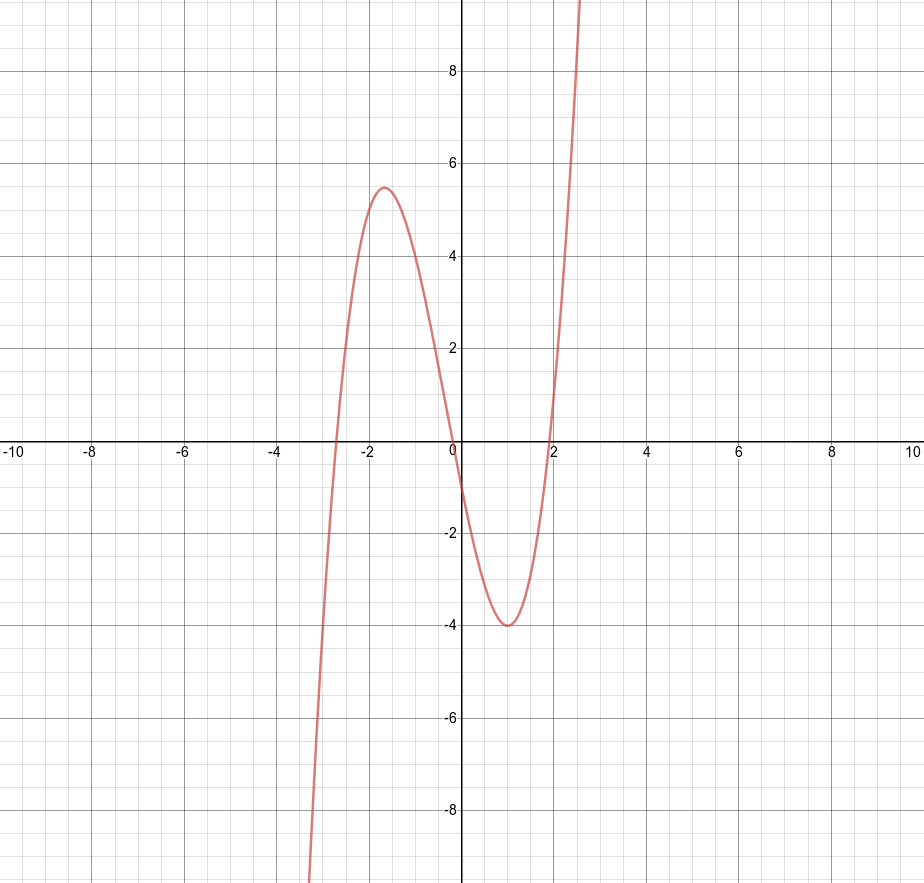
\includegraphics[scale=.3]{./diagrams/extrema1.png}
% \end{figure}

\begin{document}

\begin{frame}
  \titlepage
\end{frame}

\begin{frame}
  \frametitle{Introduction to Calculus}
\alert{Calculus} solves many problems for which it was not originally
designed. The initial motivation for calculus was to find the slope of
a tangent on a curve and the area of a region bounded by a curve.
  \begin{figure}[h]
    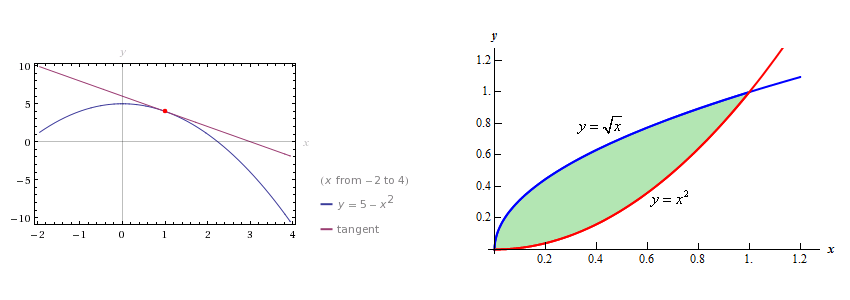
\includegraphics[scale=.35]{./diagrams/regiontangent.png}
  \end{figure}
\end{frame}

\begin{frame}
  \frametitle{A Real-Life Example I}
Consider a magnetic levitation train accelerating on a straight
monorail track. The position of the train (in feet) from the origin at
time $t$ is given by
\begin{equation}
  \label{eq:pupibahk}
  s=f(t)=4t^{2}
\end{equation}
What is the velocity of the train at $t=2$?
\end{frame}

\begin{frame}
  \frametitle{A Real-Life Example II}
It appears to make sense only if we calculate the velocity given an
interval of time rather than just one point in time. For example, the
velocity between $t=2$ and $t=3$ is 
\begin{equation}
  \label{eq:einohkie}
  v_{[2,3]}=\frac{f(3)-f(2)}{3-2}=20
\end{equation}
More generally,
\begin{equation}
  \label{eq:phaedais}
  v_{[2,t]}=g(t)=\frac{f(t)-f(2)}{t-2}=\frac{4(t^{2}-4)}{t-2}
\end{equation}
$g$ is not defined at $t=2$, but it is defined all around $t=2$, so we
can ask ourselves the question: what happens when $t\rightarrow{}2$
from below; or when $t\rightarrow{}2$ from above? It turns out that
either way, the number approaches 16.
\end{frame}

\begin{frame}
  \frametitle{Velocity at a Point}
If we found the limit as $t\rightarrow{}2$ of
\begin{displaymath}
  v_{[2,t]}=g(t)=\frac{f(t)-f(2)}{t-2}=\frac{4(t^{2}-4)}{t-2}
\end{displaymath}
it would serve as an intuitive definition of what a velocity is at a
point (instead of on an interval). Unfortunately, the limit has the
\alert{indeterminate form}
\begin{equation}
  \label{eq:toochoir}
  \lim_{t\rightarrow{}2}\frac{4(t^{2}-4)}{t-2}=\frac{0}{0}
\end{equation}
However, notice that for $t\neq{}2$,
\begin{equation}
  \label{eq:geeshaiz}
  g(t)=\frac{4(t^{2}-4)}{t-2}=\frac{4(t+2)\cancel{(t-2)}}{\cancel{t-2}}=4(t+2)
\end{equation}
\end{frame}

\begin{frame}
  \frametitle{Tangent Lines I}
Remember our magnetic levitation train. The distance-time function was
\begin{equation}
  \label{eq:leezaach}
  s=f(t)=4t^{2}
\end{equation}
The velocity of the train over a given interval is
\begin{equation}
  \label{eq:ohgheith}
  v_{[t_{1},t_{2}]}=\frac{f(t_{2})-f(t_{1})}{t_{2}-t_{1}}
\end{equation}
This velocity is also the slope of the line going through the two
function values $f(t_{1})$ and $f(t_{2})$. We call such a line a
\alert{secant line}. 
\end{frame}

\begin{frame}
  \frametitle{Tangent Lines II}
Here is an example of a secant line.
  \begin{figure}[h]
    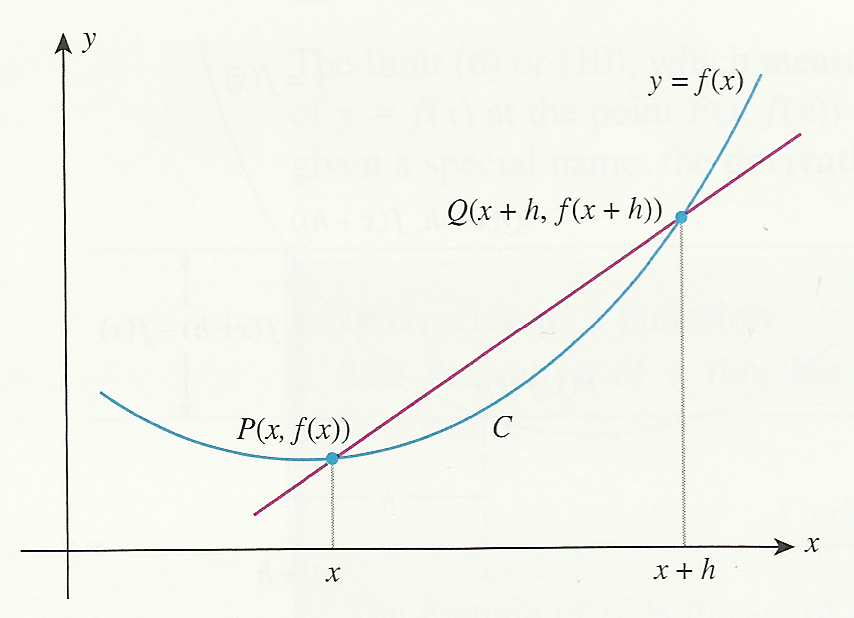
\includegraphics[scale=.7]{./diagrams/tangent2.png}
  \end{figure}
\end{frame}

\begin{frame}
  \frametitle{Tangent Lines III}
  Now imagine $t_{1}$ and $t_{2}$ moving closer and closer together at
  a point $a$ (for the train, we used $a=2$). If both of these limits
  exist and agree with each other, we have a velocity at a point,
\begin{equation}
  \label{eq:aixohshi}
  \lim_{t\rightarrow{}a}v_{[a,t]}\mbox{ for }t>a
\end{equation}
\begin{equation}
  \label{eq:oongahgh}
  \lim_{t\rightarrow{}a}v_{[t,a]}\mbox{ for }t<a
\end{equation}
This velocity at a point is also the slope of the line that just
touches the function graph without crossing it. We call it a
\alert{tangent line} at $t=a$. The slope of the tangent line is
sometimes also called the \alert{rate of change}.
\end{frame}

\begin{frame}
  \frametitle{Tangent Lines IV}
  Think of a tangent line as the limit of secant lines. The slope of a
  tangent line at a point $P=(x,f(x))$, if it exists, is
\begin{equation}
  \label{eq:cheevooj}
  \lim_{h\rightarrow{}0}\frac{f(x+h)-f(x)}{h}
\end{equation}
  \begin{figure}[h]
    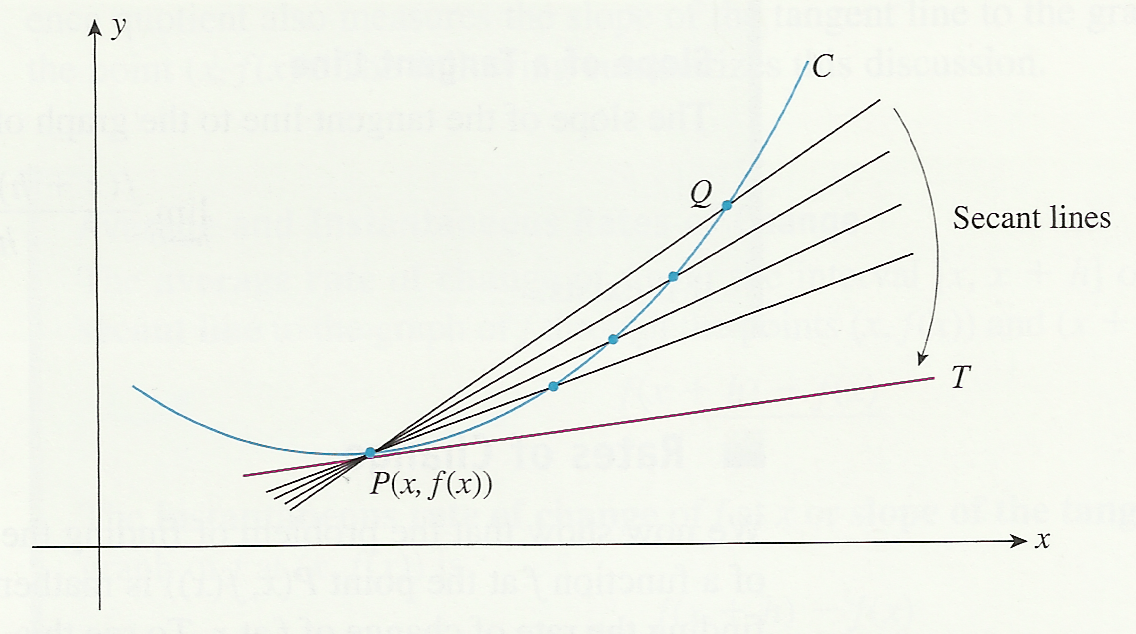
\includegraphics[scale=.7]{./diagrams/tangent1.png}
  \end{figure}
\end{frame}

\begin{frame}
  \frametitle{Derivatives}
The derivative of a function $f$ with respect to $x$ is the function
$f'$ (read ``$f$ prime''),
\begin{equation}
  \label{eq:lohfasoe}
f'(x)=\lim_{h\rightarrow{}0}\frac{f(x+h)-f(x)}{h}
\end{equation}
The domain of $f'$ is the set of all $x$ where the limit exists.
\end{frame}

\begin{frame}
  \frametitle{Derivatives Diagram I}
  \begin{figure}[h]
    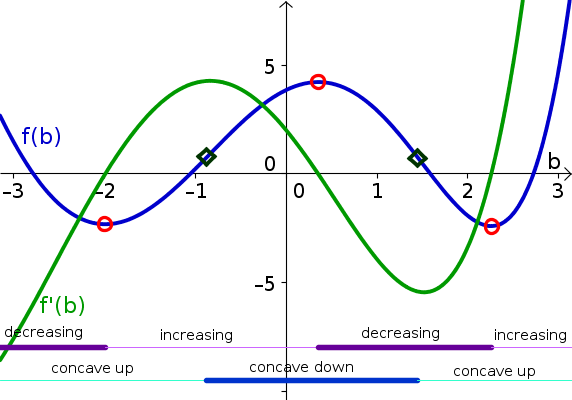
\includegraphics[scale=1.8]{./diagrams/derivs2.png}
  \end{figure}
\end{frame}

\begin{frame}
  \frametitle{Derivatives Diagram II}
  \begin{figure}[h]
    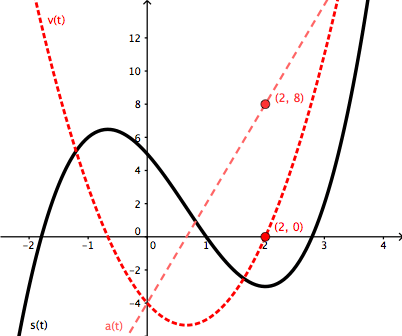
\includegraphics[scale=.6]{./diagrams/derivs1.png}
  \end{figure}
\end{frame}

\begin{frame}
  \frametitle{Basic Rules of Differentiation I}
  \begin{block}{Rule 1}
Derivative of a Constant
  \end{block}
\begin{equation}
  \label{eq:ligoovah}
f'(x)=0\mbox{ for }f(x)=c
\end{equation}
Reason:
\begin{equation}
  \label{eq:ahnieluz}
f'(x)=\lim_{h\rightarrow{}0}\frac{f(x+h)-f(x)}{h}=\lim_{h\rightarrow{}0}\frac{c-c}{h}=\lim_{h\rightarrow{}0}0=0
\end{equation}
\end{frame}

\begin{frame}
  \frametitle{Basic Rules of Differentiation II}
  \begin{block}{Rule 2}
The Power Rule
  \end{block}
\begin{equation}
  \label{eq:oomaenee}
f'(x)=nx^{n-1}\mbox{ for }f(x)=x^{n}
\end{equation}
Reason (the general case is messy, we will just show it for $f(x)=x^{2}$):
\begin{equation}
  \label{eq:eeyeejeu}
f'(x)=\lim_{h\rightarrow{}0}\frac{f(x+h)-f(x)}{h}=\lim_{h\rightarrow{}0}\frac{(x+h)^{2}-x^{2}}{h}=\notag
\end{equation}
\begin{equation}
  \label{eq:wuuxaise}
\lim_{h\rightarrow{}0}\frac{2xh+h^{2}}{h}=\lim_{h\rightarrow{}0}(2x+h)=2x
\end{equation}
\end{frame}

\begin{frame}
  \frametitle{Basic Rules of Differentiation III}
  \begin{block}{Rule 3}
Derivative of a Constant Multiple of a Function
  \end{block}
\begin{equation}
  \label{eq:thahchae}
g'(x)=c\cdot{}f'(x)\mbox{ for }g(x)=c\cdot{}f(x)
\end{equation}
Reason:
\begin{equation}
  \label{eq:quaipahn}
g'(x)=\lim_{h\rightarrow{}0}\frac{g(x+h)-g(x)}{h}=\lim_{h\rightarrow{}0}\frac{c\cdot{}f(x+h)-c\cdot{}f(x)}{h}=\notag
\end{equation}
\begin{equation}
  \label{eq:mitahrei}
\lim_{h\rightarrow{}0}c\cdot{}\frac{f(x+h)-f(x)}{h}=c\cdot\lim_{h\rightarrow{}0}\frac{f(x+h)-f(x)}{h}=c\cdot{}f'(x)
\end{equation}
\end{frame}

\begin{frame}
  \frametitle{Basic Rules of Differentiation IV}
  \begin{block}{Rule 4}
The Sum Rule
  \end{block}
\begin{equation}
  \label{eq:oubajaez}
g'(x)=f_{1}'(x)+f_{2}'(x)\mbox{ for }g(x)=f_{1}(x)+f_{2}(x)
\end{equation}
Reason:
\begin{equation}
  \label{eq:heyanaci}
g'(x)=\notag
\end{equation}
\begin{equation}
  \label{eq:bahgosio}
\lim_{h\rightarrow{}0}\frac{g(x+h)-g(x)}{h}=\lim_{h\rightarrow{}0}\frac{f_{1}(x+h)+f_{2}(x+h)-f_{1}(x)-f_{2}(x)}{h}=\notag
\end{equation}
\begin{equation}
  \label{eq:eceishie}
\lim_{h\rightarrow{}0}\left(\frac{f_{1}(x+h)-f_{1}(x)}{h}+\frac{f_{2}(x+h)-f_{2}(x)}{h}\right)=f_{1}'(x)+f_{2}'(x)
\end{equation}
\end{frame}

\begin{frame}
  \frametitle{Basic Differentiation Exercises I}
Find the derivatives for the following functions.
\begin{enumerate}
\item $f(x)=4x^{5}+3x^{4}-8x^{2}+x+3$
\item $f(t)=\frac{t^{2}}{5}+\frac{5}{t^{3}}$
\item $g(z)=2z-5\sqrt{z}$
\end{enumerate}

\bigskip

Find the slope and an equation of the tangent line to the graph of
$f(x)=2x+(1/\sqrt{x})$ at the point $(1,3)$.
\end{frame}

\begin{frame}
  \frametitle{Basic Differentiation Exercises II}
Find the derivatives for the following functions.
\begin{equation}
  \label{eq:ohzahcer}
  f(x)=5x^{\frac{4}{3}}-\frac{2}{3}x^{\frac{3}{2}}+x^{2}-3x+1
\end{equation}
\begin{equation}
  \label{eq:mothoofi}
f(x)=2t^{2}+\sqrt{t^{3}}
\end{equation}
\begin{equation}
  \label{eq:aiquooyo}
  f(x)=\frac{2}{x^{2}}-\frac{3}{x^{\frac{1}{3}}}
\end{equation}
\begin{equation}
  \label{eq:achaingo}
f(x)=\frac{3}{x^{3}}+\frac{4}{\sqrt{x}}+1
\end{equation}
\end{frame}

\begin{frame}
  \frametitle{End of Lesson}
Next Lesson: Product and Quotient Rule
\end{frame}

\end{document}
